\section{Классическая модель Барро-Гордона}
\label{sec:domain}

\paragraph{} В классической модели Барро-Гордон рассматривается власть(в виде какого-то одного политика), принимающая решение о мерах воздействия на экономику, не только на основе суммарной функции благосостояния

\begin{equation}
 \label{eq:sec:domain:main}
W=\sum_{t=0}^{\infty}\beta^t w_t = \sum_{t=0}^{\infty}\beta^t\left(y_t-\frac{\lambda\pi^2}{2}\right), 0<\beta<1
\end{equation}
где   \\   $\beta^t$ - значимость $t$-ого периода для благосотояния политика; 
\\ 
$w_t$
 -функция благосостояния политика в $t$-ом периоде;
\\ 
учитывая, что взаимосвязь между инфляцией и безработицей задается кривой Лукаса
\begin{equation}
	\label{eq:sec:domain:main1}
	y=y^*+\alpha(\pi-\pi^\beta),
\end{equation}

но и на основе того, как их оценивает население: относится оно к ним как к политикам, умеющим держать слово, или оно считает, что им нельзя доверять.
\\
Оценка населением политика в модели задается через инфляционные ожидания, которые формируются в период $t$ следующим образом:
\begin{equation}
\label{eq:sec:domain:main2}
\pi_t = \left\{ \begin{aligned} \tilde{\pi},\forall t:\pi_t=\tilde{\pi_t} 
\\ 
\frac{\alpha}{\lambda}, \exists s < t : \pi_s \ne \tilde{\pi_s} \end{aligned} \right. 
\end{equation}

где $\tilde{\pi}$ - уровень инфляции, который политики обещают достичь в результате воздействия на экономику.
\\

Как следует из ~(\ref{eq:sec:domain:main2}), если политик ведет себя честно, то население ему доверяет и ожидает тот уровень инфляции, который этот политик обещает достичь. Если политик, хотя бы раз обманул население, провел не ту политику, которую обещал, то население ему не верит, и ожидает уровень инфляции отличный от того, который этот политик обещает. Население в этом случае ожидает уровень инфляции $\frac{\alpha}{\lambda}$ , поскольку оно понимает, что в случае обмана политик будет стремиться, чтобы в экономике установился именно этот уровень инфляции.
\\

Действительно, в случае обмана политик будет выбирать уровень инфляции, который будет максимизировать его функцию благосостояния в этом периоде (допустим, в периоде $s$). Поскольку, согласно выражениям  ~(\ref{eq:sec:domain:main}) "---~(\ref{eq:sec:domain:main2}), функция благосостояния периода $s$ при $\pi_s\ne\tilde{\pi}$ имеет вид:

\begin{equation}
	\label{eq:sec:domain:main3}
	w_s=y^*\alpha\left(\pi_s - \frac{\lambda\pi^2_s}{2} \right),
\end{equation}

то уровень инфляции, максимизирующий эту функцию благосостояния , как следует из первого условия максимизации, будет равен величине $\left(\frac{\alpha}{\lambda} \right)$.
Так как репутация политика влияет на инфляционные ожидания населения, то, согласно выражениям ~(\ref{eq:sec:domain:main}) "---~(\ref{eq:sec:domain:main1}), она влияет также и на общую функцию благосостояния этого политика.
Допустим, политик ведет себя честно, то есть выполняет ту политику, которую обещал. Тогда его общая функция благосостояния

\begin{equation}
	w^{fair} = \frac{1}{(1-\beta)} \left( y^*-\frac{\lambda\pi^2}{2} \right)
\end{equation}

поскольку в этом случае для любого периода $t$, функция благосостояния периода $t$, согласно ~(\ref{eq:sec:domain:main}) "---~(\ref{eq:sec:domain:main2}), имеет вид:

\begin{equation}
w^{fair}_t = y^*-\frac{\lambda\pi^2}{2}.
\end{equation}

Если политик решит обмануть ожидания населения в какой-то период (допустим в нулевой период), то в этом случае, согласно ~(\ref{eq:sec:domain:main}) "---~(\ref{eq:sec:domain:main2}), в нулевой период его функция благосостояния будет равна

\begin{equation}
w^{deception}_0 = y^*-\frac{\alpha^2}{2\lambda}-\alpha\tilde{\pi},
\end{equation}

но во все последующее время население не будет ему доверять, поэтому его функция благосостояния в любой ненулевой период будет равна
\begin{equation}
w^{deception}_0 = y^*-\frac{\alpha^2}{2\lambda},
\end{equation}

следовательно, общая функция благосостояния политика в случае нарушения данных обещаний:

\begin{equation}
W^{deception} = \frac{1}{(1-\beta)}y^*+\frac{(1-2\beta)\alpha^2}{(1-\beta)2\lambda}-\alpha\tilde{\pi},
\end{equation}

Очевидно, что политику имеет смысл вести себя честно только в том случае, когда  $W^{fair} > W^{deception}$ , в противном случае он получит больше в случае невыполнения данных ранее обещаний.
\\

Выведем условия, при которых политик ведет себя честно, не обманывает ожидания населения. Воспользуемся для этого графической интерпретацией этой проблемы: построим графики выигрыша и проигрыша политика в случае обмана и найдем области, в которых выигрыш будет больше проигрыша и наоборот.

\begin{figure}[h]
	
	\begin{subfigure}{0.5\textwidth}
		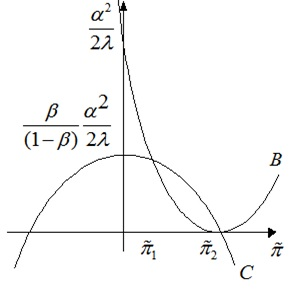
\includegraphics[width=0.9\linewidth]{pic1.jpg} 
		\caption{}
		\label{fig:pic1}
	\end{subfigure}
	\begin{subfigure}{0.5\textwidth}
		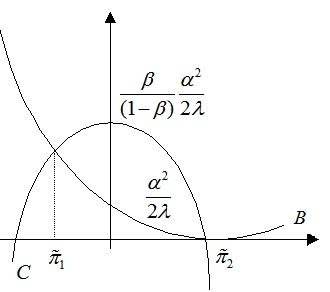
\includegraphics[width=0.9\linewidth]{pic2.jpg}
		\caption{}
		\label{fig:pic2}
	\end{subfigure}
	
	\caption{}
	\label{fig:image2}
\end{figure}

Если политик обманывает ожидание населения в нулевой момент времени, то выигрыш он получает за счет того, что в нулевой момент времени обманул ожидания населения, а проигрыш – за счет того, что в дальнейшем население перестает ему верить и всегда ожидает больший уровень инфляции, чем он объявляет.
\\

Следовательно, выигрыш обманывающего население в нулевой момент времени политика

\begin{equation}
B=w^{deception}_0 - w^{fair}_0 = \frac{\lambda\pi^2}{2}+\frac{\alpha^2}{2\lambda}-\alpha\tilde{\pi}
\end{equation}

является квадратичной функцией от объявляемого политиками уровня инфляции, который они собираются достичь. Эта функция достигает минимума $B=0$  в точке $\tilde{\pi}=\frac{\alpha}{\lambda}$, а когда $\tilde{\pi}=0$  выигрыш равен $\frac{\alpha^2}{\lambda}$.
\\

Проигрыш обманывающего население в нулевой момент времени политика также является квадратичной функцией от объявляемого политиками уровня инфляции, поскольку

\begin{equation}
	\label{eq:sec:domain:main4}
C=\sum_{t=1}^{\infty} \beta^t(w^{deception}_t - w^{fair}_t) = -\frac{\lambda\tilde{\pi}^2}{2}+\frac{\alpha^2}{2\lambda}
\end{equation}



Функция, задаваемая выражением ~(\ref{eq:sec:domain:main4}), является параболой, достигающей максимума $C=\frac{\beta}{(1-\beta)}\frac{\alpha^2}{2\lambda} $  в точке   $\tilde{\pi}=0$. Значение функции $С$ равно нулю, когда уровень инфляции   $\tilde{\pi}\pm\frac{\alpha}{\lambda}$.
\\



Взаиморасположение графиков потерь и выигрыша обманывающего население в нулевой момент времени политика зависит от того больше или меньше величина $\frac{\beta}{1-\beta}$  единицы.

Если   $\frac{\beta}{1-\beta}<1$, то есть  $\beta<\frac{1}{2}$, то функция потерь и функция выигрыша пересекаются в этом случае в точках  $\tilde{\pi}_1>0$, $\tilde{\pi}_2>0$ ~(\ref{fig:pic1}), причем  $\tilde{\pi}_1= \frac{\alpha(1-2\beta)}{\lambda}$ $\tilde{\pi}_2=\frac{\alpha}{\lambda}$. Если  $\frac{\beta}{1-\beta}>1,$  то есть  $\beta>\frac{1}{2},$  то функция потерь и функция выигрыша пересекаются в этом случае в точках   $\tilde{\pi}_1<0$, $\tilde{\pi}_2>0$ ~(\ref{fig:pic2}).
//

Таким образом из проведенного анализа следует, что поведение политика: будет он выполнять обещания или нет, зависит от его отношения к репутации. Если для политика его репутация не важна, будущее мало влияет на функцию благосостояния политика  $\beta<\frac{1}{2}$, то такому политику нет резона вести себя честно. Поскольку, как видно из ~(\ref{fig:pic1}), существует достаточно маленький уровень инфляции $\tilde{\pi}\in\left(0;\frac{\alpha(1-2\beta)}{\lambda} \right)$ , обещая который, он может получить большую реализацию своих целей в результате обмана по сравнению с честным поведением. Если для политика его репутация важна, будущее значимо для его благосостояния $\beta<\frac{1}{2}$ , то такому политику имеет смысл вести себя честно. Поскольку, как видно из  ~(\ref{fig:pic2}), не существует уровня инфляции близкого к нулю, обещая который, он может получить большую реализацию своих целей в результате обмана по сравнению с честным поведением.